\documentclass[12pt,a4paper]{ctexart}

\usepackage[a4paper,margin=2.4cm]{geometry}
\usepackage{graphicx}
\usepackage{amsmath,amssymb}
\usepackage{booktabs}
\usepackage{hyperref}
\usepackage{float}
\usepackage{longtable}
\usepackage{array}
\usepackage{caption}
\usepackage{enumitem}
\usepackage{titlesec}
\usepackage{fancyhdr}
\usepackage{xcolor}
\usepackage{setspace}
\usepackage{microtype}

\hypersetup{
  colorlinks=true,
  linkcolor=blue!50!black,
  urlcolor=blue!60!black,
  citecolor=blue!50!black,
  pdftitle={uid技术报告}
}

\setstretch{1.2}
\setlength{\parindent}{2em}
\setlength{\parskip}{0.35em}
\setcounter{tocdepth}{3}

\setlist[enumerate]{leftmargin=2.5em,itemsep=0.25em,topsep=0.35em}
\setlist[itemize]{leftmargin=2.5em,itemsep=0.25em,topsep=0.35em}

\titleformat{\section}
  {\Large\bfseries}
  {\thesection}
  {0.8em}
  {}

\titleformat{\subsection}
  {\large\bfseries}
  {\thesubsection}
  {0.8em}
  {}

\titleformat{\subsubsection}
  {\normalsize\bfseries}
  {\thesubsubsection}
  {0.8em}
  {}

\titlespacing*{\section}{0pt}{1.2em}{0.6em}
\titlespacing*{\subsection}{0pt}{0.9em}{0.4em}
\titlespacing*{\subsubsection}{0pt}{0.7em}{0.3em}

\captionsetup{
  font=small,
  labelfont=bf,
  labelsep=period
}
\renewcommand{\figurename}{Figure}

\pagestyle{fancy}
\fancyhf{}
\fancyhead[L]{Intelligent Navigation UI Technical Report}
\fancyhead[R]{\thepage}
\renewcommand{\headrulewidth}{0.4pt}

\begin{document}

\begin{titlepage}
  \centering
  \vspace*{2.5cm}
  {\zihao{2}\bfseries uid技术报告\par}
  \vspace{1cm}
  {\zihao{3}\bfseries Intelligent Navigation UI Technical Report\par}
  \vspace{2.2cm}

  \renewcommand{\arraystretch}{1.45}
  \begin{tabular}{>{\bfseries}p{4cm}p{8cm}}
    Course: & ISE 333: User Interface Development (Design) \\
    Project Title: & An Intelligent Navigation UI \\
    Instructor: & Hao Li \\
    Semester: & Spring 2026 \\
  \end{tabular}

  \vspace{0.9cm}
  {\bfseries GitHub Repository: }{\url{https://github.com/EDLlyc/Intelligent-Navigation-UI}\par}

  \vspace{1.8cm}

  {\bfseries Group Members: \par}
  \vspace{0.7cm}

  \begin{tabular}{p{6cm}p{4cm}}
    李昱辰 & R32314003 \\
    纪玮祺 & R32314005 \\
    王瑞尧 & R32314007 \\
    刘江翰 & R32314009 \\
    刘熙鹏 & R32314091 \\
  \end{tabular}

  \vfill
\end{titlepage}

\tableofcontents
\clearpage

\section{Project Overview}

This project implements an Intelligent Navigation UI in MATLAB. The system uses the provided map image MapForUI.jpg and allows users to perform navigation-related operations through a graphical user interface. Running main.m launches the UI directly.

Basic settings of the system are as follows:

Map image: MapForUI.jpg

Image size: 803 x 1404 pixels

Scale: 1 pixel = 1.7 meters

Real-world origin: bottom-left corner

IV size: 8 m x 3 m

The project implements all required basic functions and all five optional functions in one unified UI.

\section{System Design Idea}

\subsection{Overall Design}

The system is built around a MATLAB GUI. It includes a main map area, a right-side control panel, measurement tools, map rotation tools, and tabs for optional functions. The whole system is started by running main.m.

\subsection{Coordinate System Design}

The real-world coordinate system uses the bottom-left corner of the map as the origin. Pixel coordinates are converted into real-world coordinates using the scale 1.7 m/pixel. This conversion is used for coordinate display, IV placement, distance calculation, trajectory calculation, and path planning.

\subsection{Road Validity Checking}

The system checks whether a clicked point is on the road before performing operations such as loading an IV or using optional functions. If the point is invalid, the UI shows an error message. If the point is valid, the operation continues.

\subsection{Intelligent Vehicle Representation}

Each IV is represented as a rectangle of size 8 m x 3 m. The system stores its ID, real-world position, heading angle, and scale factor. The UI supports loading, selecting, removing, and reporting multiple IVs.

\subsection{Interaction Design}

The system is event-driven. Most operations are triggered by clicking buttons, clicking points on the map, and switching optional-function tabs. After startup, normal user operations are completed through the UI.

\section{Basic UI Requirements}

\subsection{Launching the UI}

The system is launched by running main.m. After startup, users perform all normal operations through the GUI.

\begin{figure}[H]
  \centering
  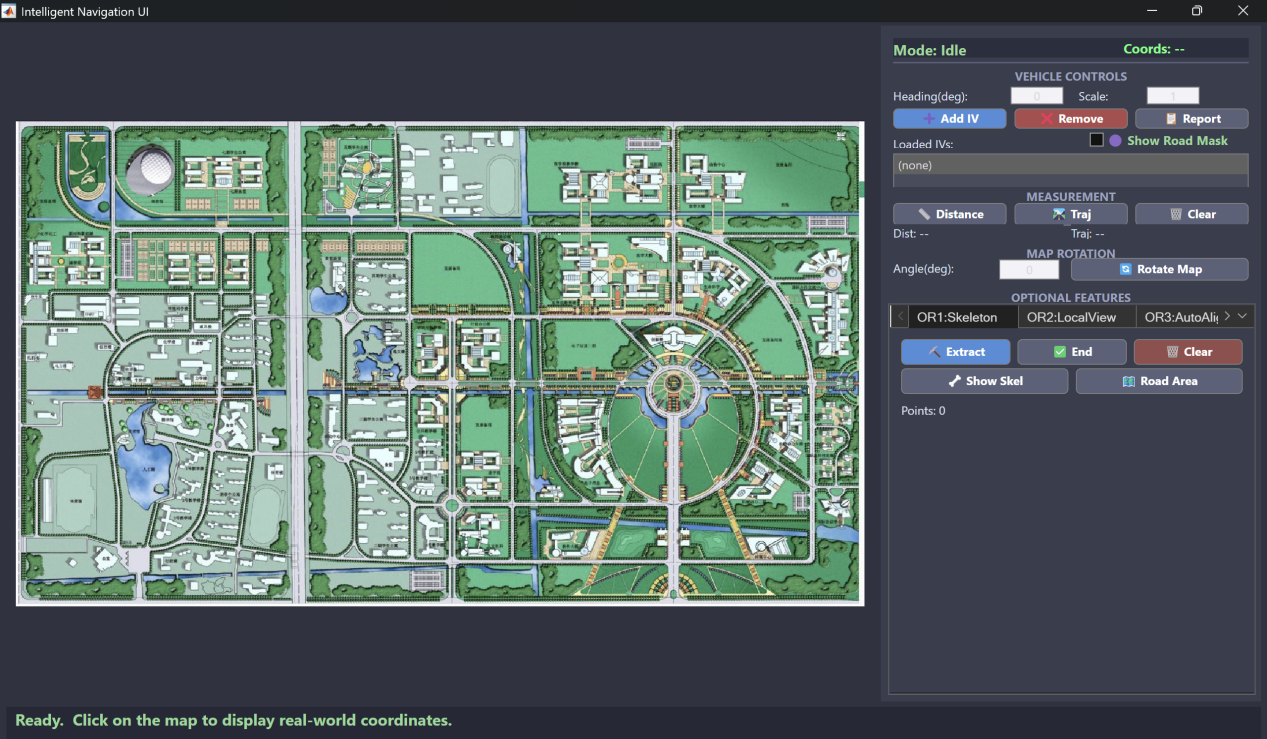
\includegraphics[width=0.92\textwidth]{uid_report_images/image_02.png}
  \caption{Main interface after startup.}
  \label{fig:main-ui}
  \caption*{Note: This figure shows the complete main interface after startup. The left side is the main map area, and the right side is the control panel for IV operations, measurement, map rotation, and optional functions. The status bar at the bottom shows system prompts and messages.}
\end{figure}

\subsection{Map Loading and Visualization}

The map image is loaded and displayed in the main visualization area of the UI.

\subsection{Displaying Real-World Coordinates}

When the user clicks a point on the map, the system displays its real-world coordinates.

\subsection{Loading One or Multiple IVs}

The UI allows the user to add one or more IVs onto the map.

\subsection{Adjustable IV Orientation}

Before placing an IV, the user can input its heading angle through the UI.

\begin{figure}[H]
  \centering
  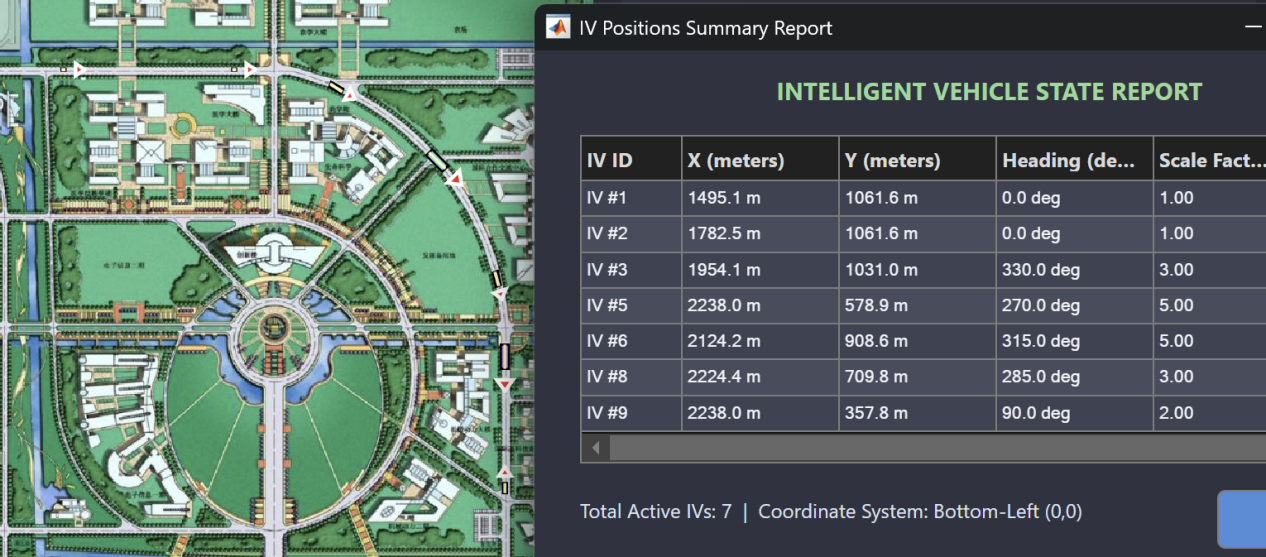
\includegraphics[width=0.92\textwidth]{uid_report_images/image_04.png}
  \caption{Interface after loading multiple IVs.}
  \label{fig:multi-iv}
  \caption*{Note: This figure shows the interface after multiple IVs have been loaded. The map displays several IVs at different positions and headings, and the report window lists their IDs, real-world coordinates, heading angles, and scale factors.}
\end{figure}

\subsection{Road Validity Check \& Road Detection Algorithm}

\subsubsection{Road Validity Checking Mechanism (Runtime)}

Before loading an Intelligent Vehicle (IV) or executing dependent operations (such as path planning), the system must validate whether the user-clicked point falls on a navigable road. The runtime check sequence is designed as follows:

\begin{enumerate}
  \item \textbf{Coordinate Mapping}: The user's interaction coordinate on the GUI canvas is mapped into the corresponding pixel index $(r, c)$ of the map image matrix.
  \item \textbf{Mask Querying}: The pre-computed binary road mask matrix (\texttt{roadMask}) is queried at the exact row and column location:
  \item $\text{isValid} = \text{roadMask}(r, c)$
  \item \textbf{Execution Decision}: If the queried value is \texttt{true}, the point is accepted, and the IV placement or navigation operation continues. If the value is \texttt{false}, the operation is intercepted, and an explicit error message is displayed in the UI status bar to notify the user.
\end{enumerate}

\subsubsection{Multi-Stage Road Detection Algorithm (Offline Pipeline)}

To ensure real-time responsiveness during runtime without relying on any advanced MATLAB Toolboxes (satisfying the project's hard constraints), the binary road mask is generated offline using a custom \textbf{Multi-Stage Pixel Classification \& Morphological Refinement Algorithm}. The complete image processing pipeline consists of the following 8 stages:

\paragraph{HSV-Space Dual-Channel Color Filtering (Path A)}

The primary road surface (asphalt and concrete) exhibits low saturation and moderate brightness. Without using any high-level toolbox functions, the saturation ($S$) and brightness ($V$) channels are derived manually from the raw RGB channels:

\[
S = \frac{\max(R,G,B) - \min(R,G,B)}{\max(R,G,B)}, \quad V = \max(R,G,B)
\]

A pixel is classified as a preliminary road candidate if it satisfies:

\[
S < 0.22 \quad \land \quad 0.55 < V < 0.95 \quad \land \quad B < G + 0.10 \quad \land \quad G < R + 0.07
\]

To eliminate bright-white building roofs and uniform highly-reflective grey surfaces, two exclusive constraints are enforced (where $C = \frac{R+G+B}{3}$):

\[
\neg (V > 0.85 \land S < 0.08) \quad \land \quad \neg (C > 0.78 \land S < 0.12)
\]

\paragraph{Reference-Colour Distance Rescue (Path B)}

Certain road segments with distinctive teal-grey tones or those affected by specific atmospheric illumination are prone to being missed by the fixed thresholds of Path A. To improve the recall rate, a parallel rescue path computes the minimum Euclidean distance in the RGB color space from the current pixel to a set of eight hand-picked baseline road color samples $\{(R_k, G_k, B_k)\}_{k=1}^8$:

\[
d_{\min} = \min_{k} \sqrt{(R - R_k)^2 + (G - G_k)^2 + (B - B_k)^2}
\]

Pixels with $d_{\min} < 0.08$ that conform to fundamental intensity bounds are safely recalled and merged ($\cup$) with the candidates from Path A.

\paragraph{Local Adaptive Shadow Recovery}

Road areas occluded by tree canopies or building shadows suffer from significant illumination dropouts. The algorithm implements a local adaptive rescue mechanism. An integral image is constructed manually to efficiently compute the local brightness mean $V_{\text{local}}$ within a $31 \times 31$ sliding window. Pixels whose local brightness ratio falls within an empirically verified road-shadow interval are classified as road pixels, successfully resolving shadow-induced road fragmentation.

\paragraph{Morphological Closing Refinement}

To bridge pixel-level micro-fractures inside the road areas and smooth the jagged boundaries caused by noise, a morphological closing operation (dilation followed by erosion) is performed. A circular structuring element with a radius of 2 pixels is implemented using basic array shifting and logical operations, avoiding toolbox dependencies.

\paragraph{Neighbourhood Majority Filtering}

To eliminate isolated salt-and-pepper noise and fine pixel-level burrs at the edges, a strict 8-neighbourhood majority filter is applied. For each candidate road pixel, the number of its 8 neighbours that are also marked as road is counted. The pixel is retained if and only if:

\[
N_{\text{road\_neighbours}} \ge N_{\min} \quad (\text{where } N_{\min} = 2)
\]

\paragraph{Solidity-Based Building Rejection}

Some building roofs share identical spectral signatures with road materials. Since building contours are typically compact and solid rectangles whereas roads are winding, narrow, and elongated, they can be distinguished via geometric features. The algorithm utilizes a custom 8-connected Breadth-First Search (BFS) to label all independent connected components. For each component $C_i$, its solidity is evaluated against its bounding box:

\[
\text{Solidity}(C_i) = \frac{|C_i|}{\text{BoundingBoxHeight}(C_i) \times \text{BoundingBoxWidth}(C_i)}
\]

Components representing large buildings exhibit high solidity and are completely filtered out by enforcing a strict upper bound: $\text{Solidity}(C_i) \le 0.20$.

\paragraph{BFS Connectivity Main-Network Filtering}

To erase fragmented false-positive clusters scattered across the map (such as parking lots, isolated concrete paths, or unresolved backyard patches), a final connectivity filter is applied. A standard 8-connected BFS flood-fill originates from a known, guaranteed main-road seed pixel at coordinate $(517, 468)$. Only the massive connected component linked to this seed is preserved, completely wiping out all disjointed false-positive regions.

\paragraph{Black-and-White List Hardcoded Correction}

To achieve a flawless road mask for runtime robustness, the algorithm automatically cross-references its generated mask against a manually traced, pixel-perfect ground-truth road path drawn in Adobe Photoshop at the identical $803 \times 1404$ resolution.

\begin{itemize}
  \item Remaining micro-scale false positives are compiled into a deterministic \textbf{Blacklist} database.
  \item Micro-scale false negatives are compiled into a \textbf{Whitelist} database.
\end{itemize}

During the final offline export, these database tables are used to hardcode corrections over the mask matrix, resolving the remaining 3.34\% of classification errors.

\subsubsection{Quantitative Evaluation}

The optimal hyperparameters ($S_{\max}=0.22$, $V_{\min}=0.55$, $V_{\max}=0.95$, $\text{Solidity}_{\max}=0.20$, and $N_{\min}=2$) were determined using a grid search to maximize the $F_1$ score against the Photoshop-annotated reference.

Prior to the hardcoded database correction, the automated pipeline achieved an excellent performance with \textbf{Precision = 96.66\%}, \textbf{Recall = 100.00\%}, and an \textbf{Intersection over Union (IoU) = 96.66\%} ($F_1\text{-score} = 98.30\%$). Following the execution of the Black-and-White list correction, the final pre-computed road mask delivers a \textbf{100\% zero-error exact match} to the map infrastructure, guaranteeing absolute precision for the runtime UI navigation.

\begin{figure}[H]
  \centering
  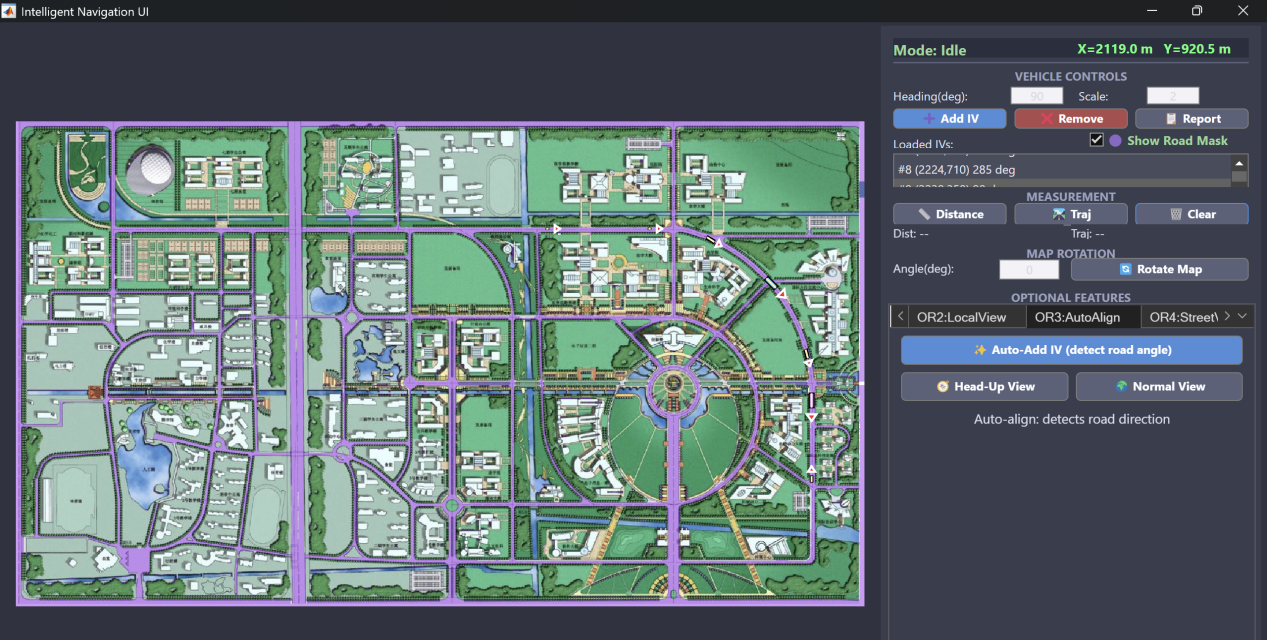
\includegraphics[width=0.92\textwidth]{uid_report_images/image_03.png}
  \caption{Road mask display after enabling Show Road Mask.}
  \label{fig:road-mask}
  \caption*{Note: This figure shows the result after enabling Show Road Mask.}
\end{figure}

\subsection{Removing IVs}

The UI allows the user to remove one selected IV without affecting other loaded IVs.

\subsection{Reporting All Loaded IV Positions}

The UI provides a function to report the real-world positions of all currently loaded IVs.

\subsection{Measuring Real-World Distance Between Two Points}

The system supports measuring the real-world distance between two clicked points on the map.

\begin{figure}[H]
  \centering
  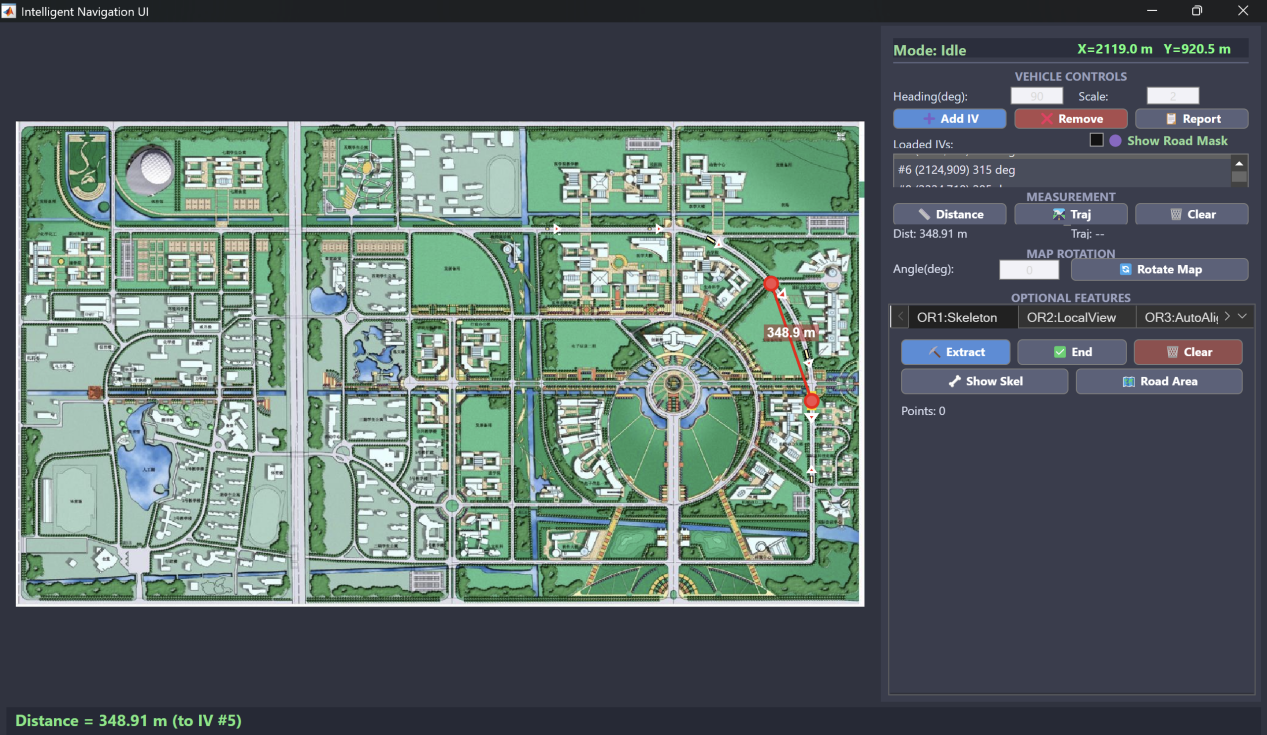
\includegraphics[width=0.92\textwidth]{uid_report_images/image_05.png}
  \caption{Distance measurement between two selected points.}
  \label{fig:distance}
  \caption*{Note: This figure shows the distance measurement function between two selected points on the map. The system draws a segment between the two points and displays the measured real-world distance on the map and in the right panel. This figure shows that the UI supports interactive two-cars distance measurement.}
\end{figure}

\subsection{Measuring Trajectory Length}

The system supports continuous clicking on the map to form a trajectory and calculate its total real-world length.

\begin{figure}[H]
  \centering
  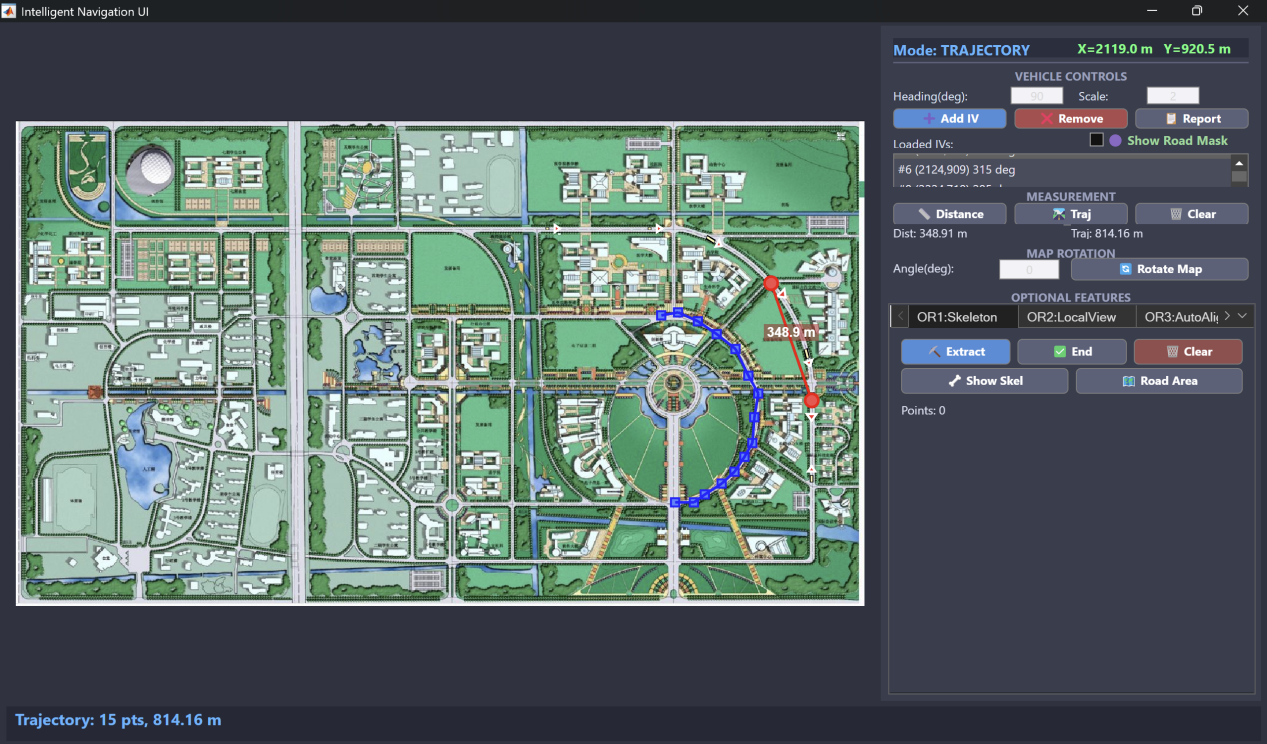
\includegraphics[width=0.92\textwidth]{uid_report_images/image_06.png}
  \caption{Trajectory measurement result.}
  \label{fig:trajectory}
  \caption*{Note: This figure shows the trajectory measurement function. The system records multiple clicked points, draws the trajectory on the map, and displays the total real-world trajectory length in the right panel.}
\end{figure}

\subsection{Map Rotation}

The user can input a rotation angle, and the system displays the rotated map accordingly.

\begin{figure}[H]
  \centering
  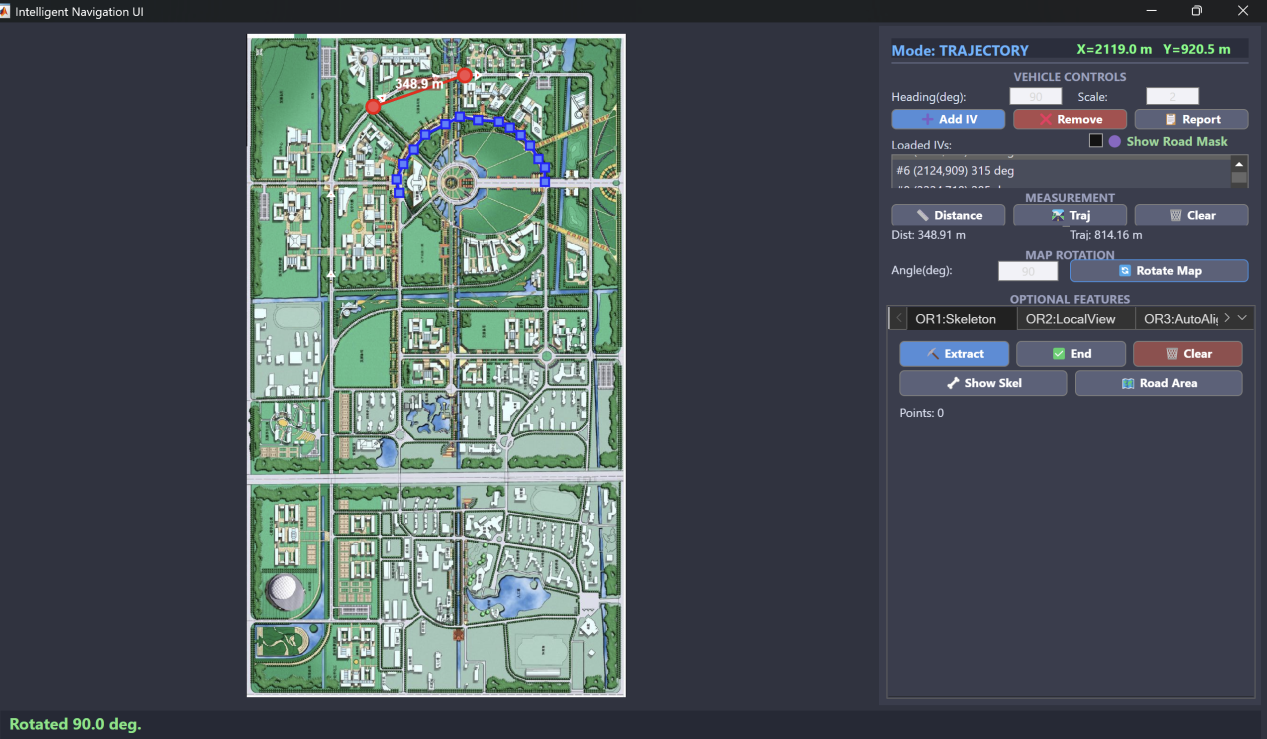
\includegraphics[width=0.92\textwidth]{uid_report_images/image_07.png}
  \caption{Map after a 90-degree rotation.}
  \label{fig:rotation}
  \caption*{Note: This figure shows the map after a 90-degree rotation. The rotated map is displayed in the main area, and the control panel remains available for further operations. This figure shows that the system supports map rotation and keeps the related measurement results visible after rotation.}
\end{figure}

\section{Optional Requirements}

\subsection{OR1: Road Skeleton Extraction}
\label{sec:or1}

\textbf{Responsible member: 刘熙鹏 R32314091}

Function description:

Supports manual extraction of a road skeleton by clicking valid road pixels on the main map, and provides skeleton-based visualization in the UI.

Implementation idea:

The OR1 panel allows the user to click a sequence of road points as skeleton control points. Each click is validated using the pre-computed binary road mask. The extracted skeleton is stored as an ordered polyline and can be visualized either as (1) the skeleton itself or (2) a road region attached to the skeleton.

Key parameters / data:

Map resolution: $s = 1.7$ m/pixel

Road mask: \texttt{roadMask} (binary, pre-computed)

Skeleton neighbourhood radius (for road-area visualization): $R$ meters (user-defined or fixed), $r = \lceil R/s \rceil$ pixels

Processing pipeline:

\begin{enumerate}
  \item Input acquisition

  User click coordinate on the main map: $(u_i, v_i)$ in map-image pixel coordinates.

  \item Validity check (road-only constraint)

  Accept the click only if $\text{roadMask}(v_i, u_i) = \text{true}$. Otherwise show an error.

  \item Skeleton recording

  Append $(u_i, v_i)$ into an ordered list $S = \{(u_1, v_1), \dots, (u_n, v_n)\}$.

  \item Visualization A: Skeleton overlay

  Render the polyline by connecting consecutive skeleton points.

  \item Visualization B: Road area attached to skeleton

  Convert $R$ meters to $r$ pixels.

  For each skeleton point, take the disk neighbourhood and union all neighbourhoods:

  \[
  \Omega = \bigcup_i \{(u,v)\mid (u-u_i)^2+(v-v_i)^2 \le r^2\}
  \]

  Display $\text{roadMask} \cap \Omega$ as the related road area.
\end{enumerate}

How to use:

\begin{enumerate}
  \item Open OR1 tab → Click Extract
  \item Click multiple road points → Click End
  \item Click Show Skel to display skeleton polyline
  \item Click Road Area to display skeleton-attached road region
  \item Click Clear to reset
\end{enumerate}

Representative results of OR1 are shown in Figures~\ref{fig:or1a} and \ref{fig:or1b}.

\begin{figure}[H]
  \centering
  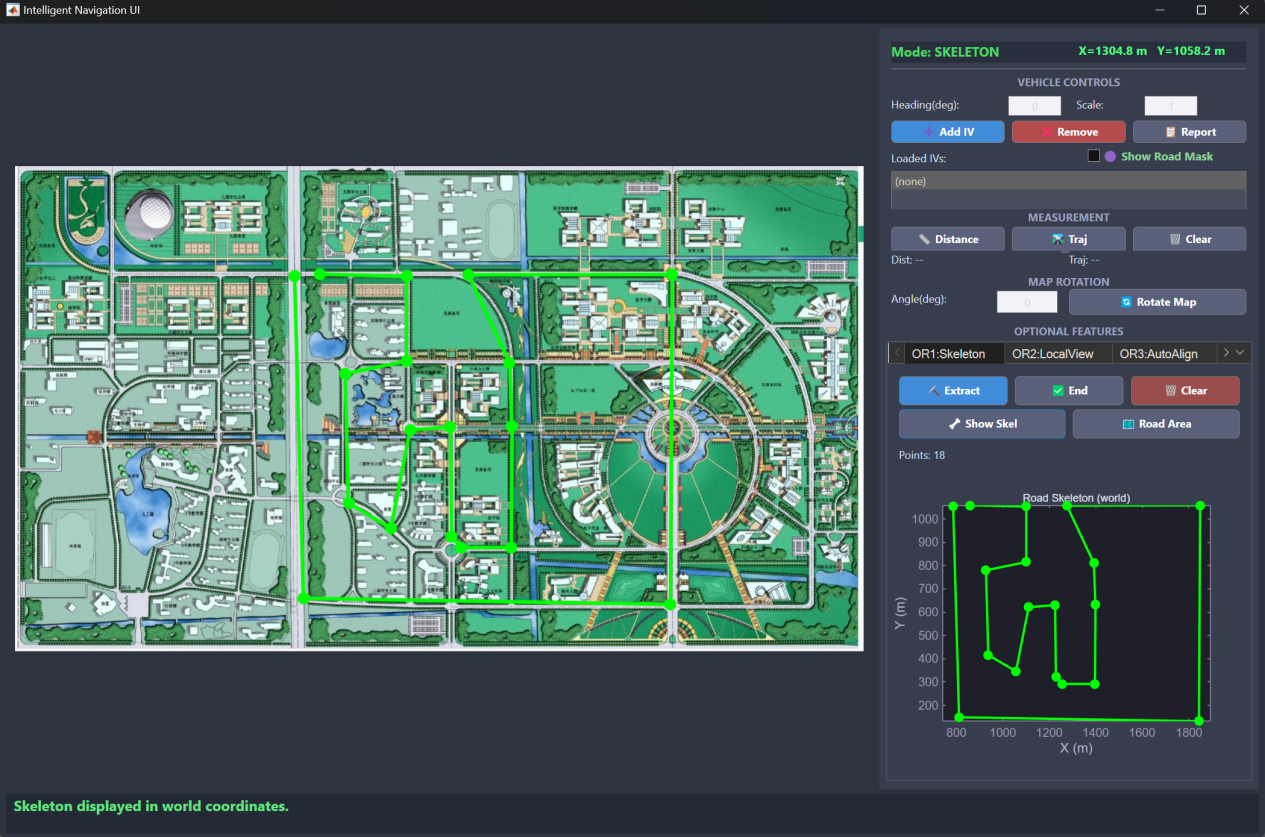
\includegraphics[width=0.92\textwidth]{uid_report_images/image_08.png}
  \caption{OR1 result: extracted skeleton in world coordinates.}
  \label{fig:or1a}
\end{figure}

\begin{figure}[H]
  \centering
  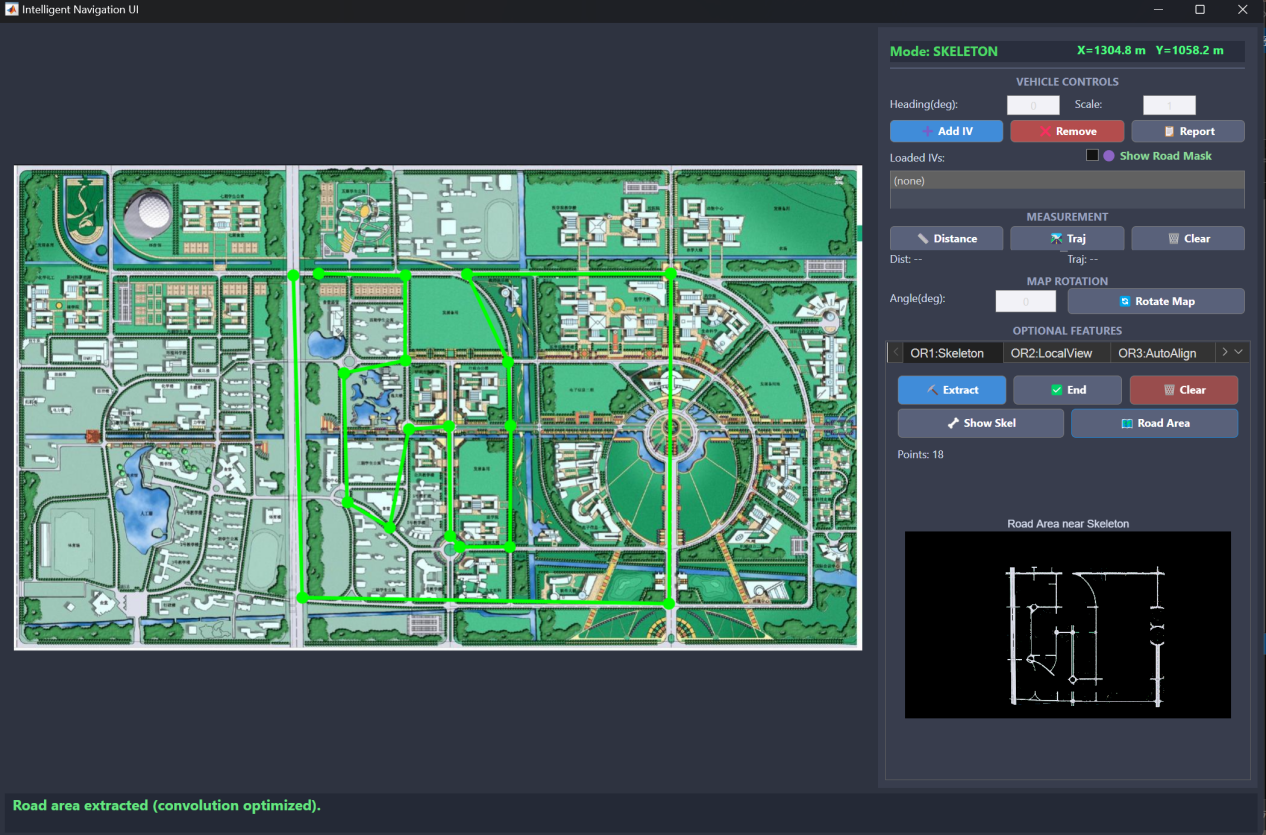
\includegraphics[width=0.92\textwidth]{uid_report_images/image_09.png}
  \caption{OR1 result: road region related to the selected skeleton.}
  \label{fig:or1b}
  \caption*{Note: These figures show the OR1 results. The upper image shows the extracted skeleton visualized in world coordinates, and the lower image shows the road region related to the selected skeleton.}
\end{figure}

\subsection{OR2: Scale and Local Visualization}
\label{sec:or2}

\textbf{Responsible member: 刘江翰 R32314009}

Function description:

Provides a circular local map view centered at a selected IV, and supports scale-based rendering of the IV on that local view.

Implementation idea:

The OR2 panel extracts a circular local region around the selected IV using a user-specified range in meters. The IV marker is rendered according to its scale factor. A direction indicator can be toggled.

Key parameters / data:

Map resolution: $s = 1.7$ m/pixel

Local range: $R$ meters $\rightarrow$ radius in pixels $r = \lceil R/s \rceil$

IV scale factor: $k$ (user-defined or internal)

Optional heading: $\theta$

Processing pipeline:

\begin{enumerate}
  \item IV selection

  Choose an IV with world position $(x,y)$ and heading $\theta$.

  \item World $\rightarrow$ map pixel mapping

  Convert $(x,y)$ into map pixel center $(u_c, v_c)$ using the system’s coordinate mapping.

  \item Range conversion

  $r = \lceil R/s \rceil$.

  \item ROI extraction + circular mask

  Extract square ROI around $(u_c, v_c)$: $[u_c - r, u_c + r] \times [v_c - r, v_c + r]$.

  Apply circular mask: keep pixels satisfying $(u - u_c)^2 + (v - v_c)^2 \le r^2$.

  \item IV rendering with scale

  Render IV marker at local-view center with size proportional to $k$.

  \item Direction indicator (optional)

  If enabled, draw a heading arrow with direction $\theta$.
\end{enumerate}

How to use:

\begin{enumerate}
  \item Load IV(s) $\rightarrow$ Select one IV
  \item Open OR2 tab $\rightarrow$ Input range $R$ meters
  \item Click Update
  \item Click Show Direction to toggle heading display
\end{enumerate}

Representative results of OR2 are shown in Figures~\ref{fig:or2a} and \ref{fig:or2b}.

\begin{figure}[H]
  \centering
  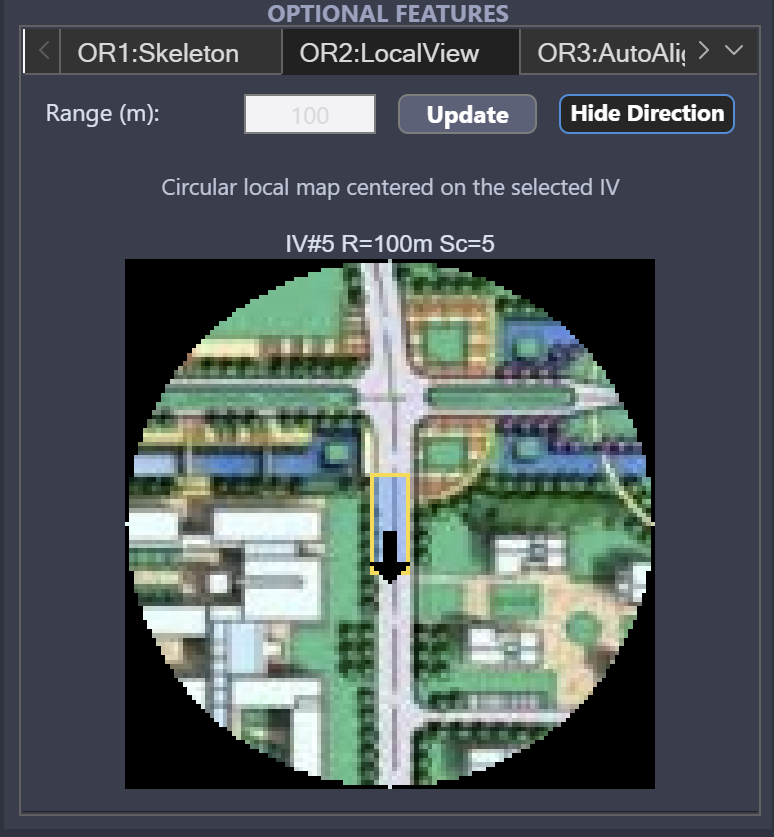
\includegraphics[width=0.92\textwidth]{uid_report_images/image_10.png}
  \caption{OR2 result: local circular map with direction display enabled.}
  \label{fig:or2a}
\end{figure}

\begin{figure}[H]
  \centering
  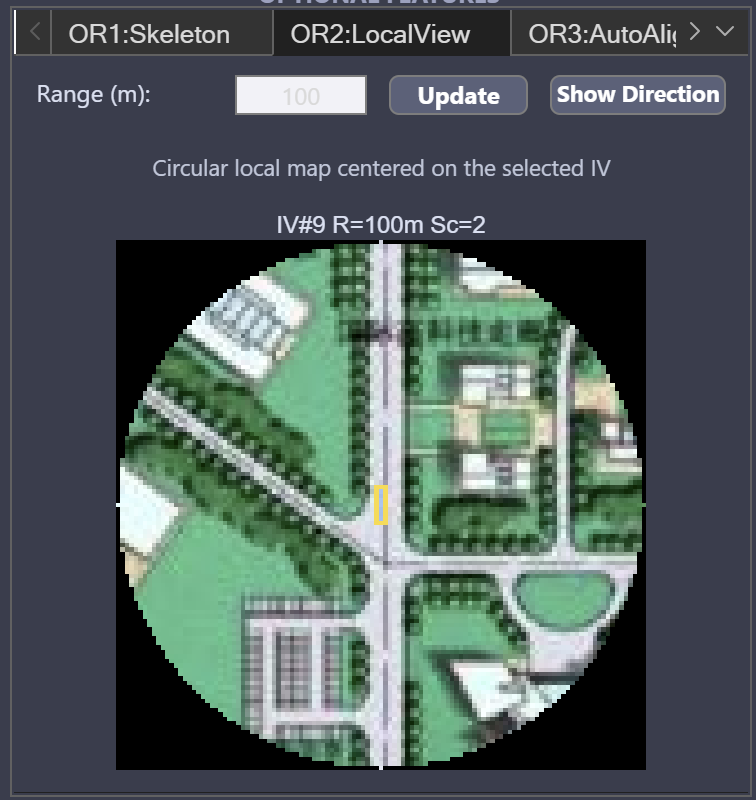
\includegraphics[width=0.92\textwidth]{uid_report_images/image_11.png}
  \caption{OR2 result: local circular map with direction display hidden.}
  \label{fig:or2b}
  \caption*{Note: This figure shows the OR2 local circular map visualization. The local view is centered on the selected IV and is displayed according to the user-defined range. The left image shows the case when the direction display is enabled, and the right image shows the case when the direction display is hidden.}
\end{figure}

\subsection{OR3: IV Automatic Orientation Alignment}
\label{sec:or3}

\textbf{Responsible member: 王瑞尧 R32314007}

Function description:

Loads an IV with heading automatically aligned to the local road direction, and supports head-up view where the selected IV always faces upward.

Implementation idea:

After the user clicks a road point, the system estimates the dominant local road direction around that pixel by analysing nearby road pixels in the binary road mask. The estimated direction is assigned as the IV heading. In head-up view, the map is rotated so the IV’s heading aligns with upward screen direction.

Key parameters / data:

Road mask: \texttt{roadMask}

Neighbourhood window radius: $w$ pixels (e.g. $w = 10$, window size $2w + 1$)

Heading angle: $\theta$

Head-up target direction: $\theta_\text{up}$ (screen upward direction convention)

Processing pipeline:

A) Auto heading estimation

\begin{enumerate}
  \item Input and validation

  User click $(u_0, v_0)$, accept only if $\text{roadMask}(v_0, u_0)=\text{true}$.

  \item Neighbourhood sampling

  Collect all road pixels within window:

  \[
  P=\{(u,v)\mid |u-u_0|\le w,\ |v-v_0|\le w,\ \text{roadMask}(v,u)=\text{true}\}
  \]

  \item Dominant direction estimation (PCA-based)

  Compute covariance of points in $P$; the principal eigenvector $\vec{d}$ is the dominant direction.

  Convert to heading angle: $\theta = \text{atan2}(d_y, d_x)$.

  \item Assign IV heading

  Set IV heading = $\theta$ and load IV.
\end{enumerate}

B) Head-up view rotation

\begin{enumerate}
  \item Compute rotation angle

  \[
  \Delta = \theta_\text{up} - \theta_\text{IV}
  \]

  \item Rotate map rendering

  Rotate the map around the selected IV’s screen position by $\Delta$, keeping the IV state consistent.
\end{enumerate}

How to use:

\begin{enumerate}
  \item Open OR3 tab $\rightarrow$ Click Auto-Add IV
  \item Click a road point to add an IV with auto heading
  \item Select an IV $\rightarrow$ Click Head-Up View / Normal View
\end{enumerate}

Representative results of OR3 are shown in Figures~\ref{fig:or3a} and \ref{fig:or3b}.

\begin{figure}[H]
  \centering
  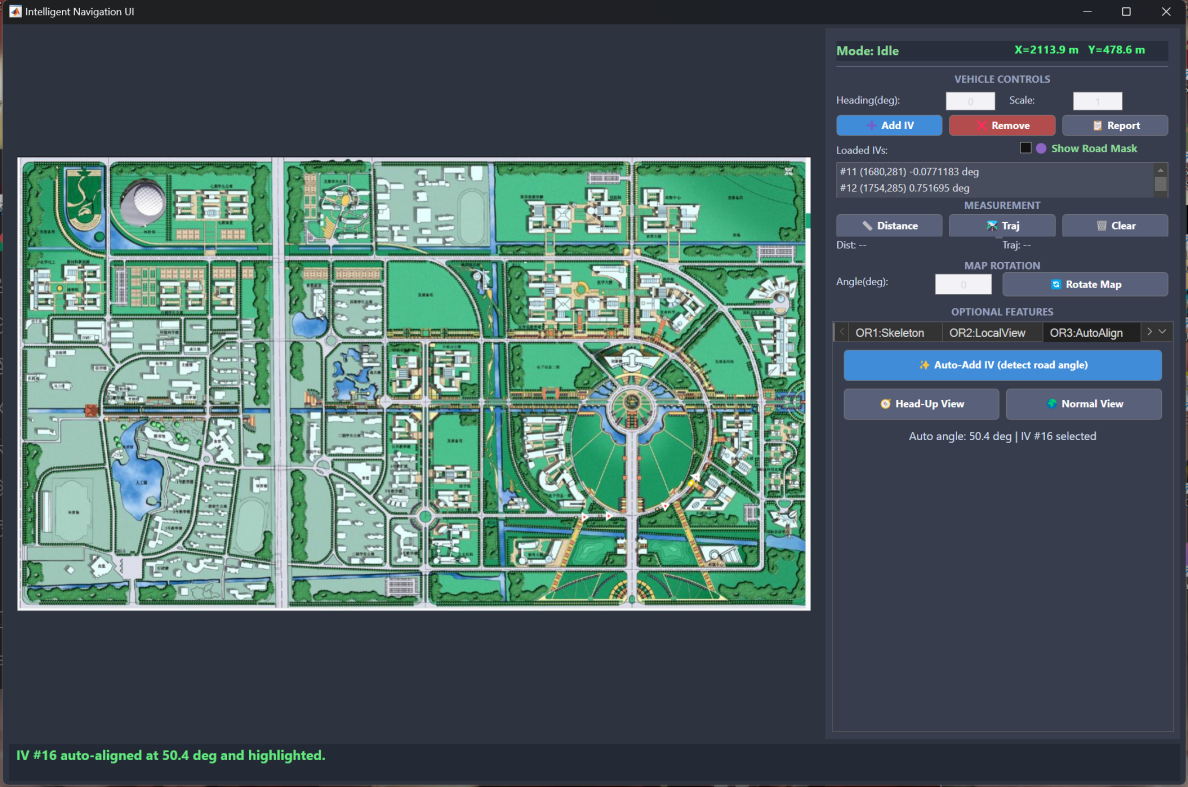
\includegraphics[width=0.92\textwidth]{uid_report_images/image_12.png}
  \caption{OR3 result: automatic heading alignment based on local road direction.}
  \label{fig:or3a}
\end{figure}

\begin{figure}[H]
  \centering
  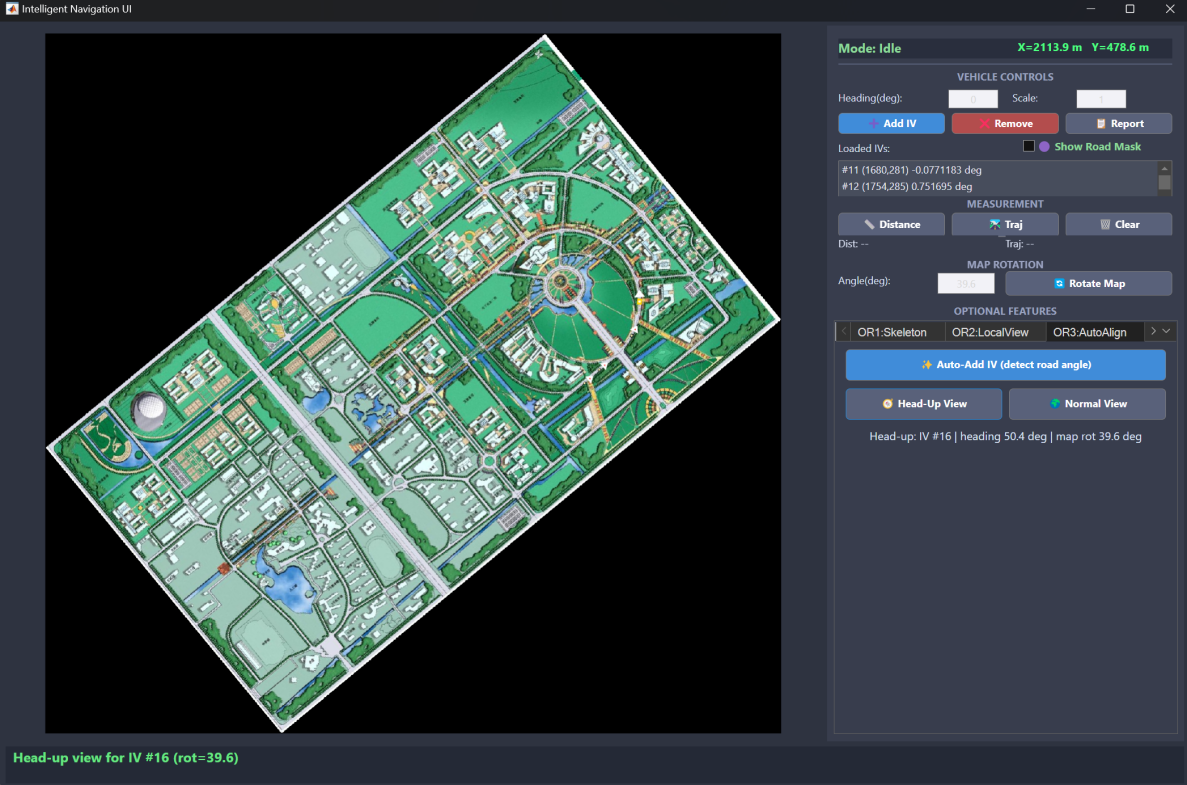
\includegraphics[width=0.92\textwidth]{uid_report_images/image_13.png}
  \caption{OR3 result: Head-Up View with the selected IV facing upward.}
  \label{fig:or3b}
  \caption*{Note: This figure shows the OR3 functions. The upper image shows automatic heading alignment based on the local road direction. The lower image shows the Head-Up View, where the map is rotated so that the selected IV faces upward. This figure demonstrates the main functions of OR3.}
\end{figure}

\subsection{OR4: Virtual Street View Generation}
\label{sec:or4}

\textbf{Responsible member: 纪玮祺 R32314005}

Function description:

Generates a pseudo-3D perspective street view from a 2D map at a given road coordinate, showcasing a forward-extending road, gradient sky, and distance-based fog.

Implementation idea:

The system implements backward homography mapping (ray casting) to map ground coordinates to screen pixels.

\begin{enumerate}
  \item Camera parameters:
\end{enumerate}

Output size: W = 500, H = 400 pixels.

Center main point: (u0, v0) = (250, 200).

Focal length: f = 330.0.

Camera height: $Zc$ = 1.6 meters.

Pitch angle: pitch = -10.0 degrees.

Yaw angle: yaw = 90 - roadAngle.

Intrinsic Matrix: $A = [330, 0, 250; 0, 330, 200; 0, 0, 1]$.

\begin{enumerate}
  \item Backward projection chain (ICS -> CCS -> WCS -> Map):
\end{enumerate}

ICS to CCS ray direction: $Pc = A^{-1} * Pi$ where $Pi = [u, v, 1]^T$

CCS to WCS ray rotation: $rays_w = R_{cw} * Pc$, where $R_{cw} = [u_c, v_c, n_c]$ is the rotation matrix constructed from Yaw and Pitch.

WCS ground intersection: Since $Zw = 0$, the ray parameter $t = -Oc(3) / rays_w(3)$.

WCS point: $Pw = Oc + t * rays_w$.

Map pixel mapping: $u_{map} = Pw(1)/scale + 0.5$, $v_{map} = mapHeight - Pw(2)/scale + 0.5$.

Texturing: Sample color at $(u_{map}, v_{map})$ on the 2D map.

How to use:

\begin{enumerate}
  \item Select the "StreetView" tab (OR-4)
  \item click the "Generate Street View" button
  \item click on any \textbf{road point} on the main map.
\end{enumerate}

Representative results of OR4 are shown in Figures~\ref{fig:or4a}, \ref{fig:or4b}, and \ref{fig:or4c}.

\begin{figure}[H]
  \centering
  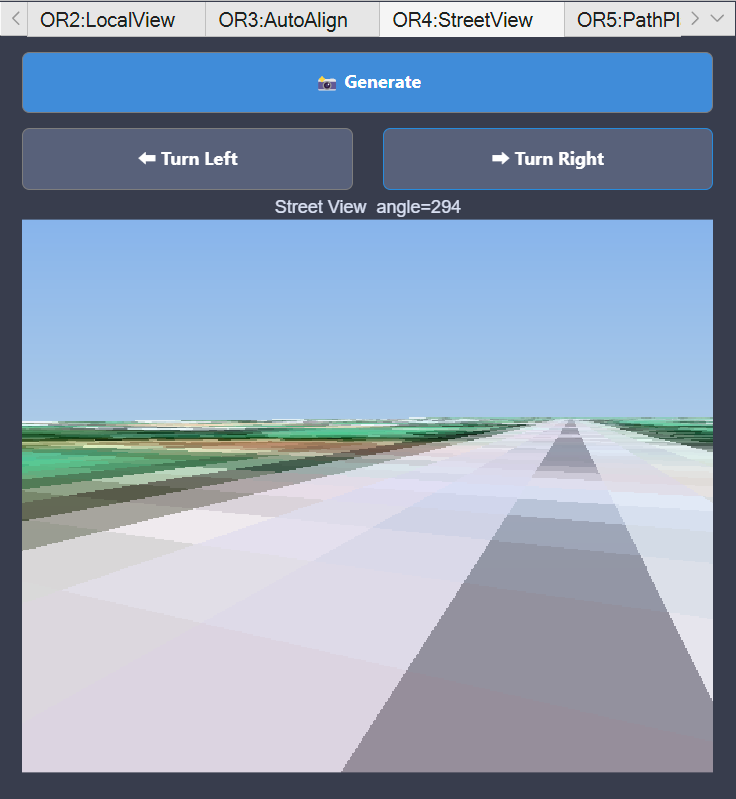
\includegraphics[width=0.92\textwidth]{uid_report_images/image_14.png}
  \caption{OR4 result: original virtual street view.}
  \label{fig:or4a}
\end{figure}

\begin{figure}[H]
  \centering
  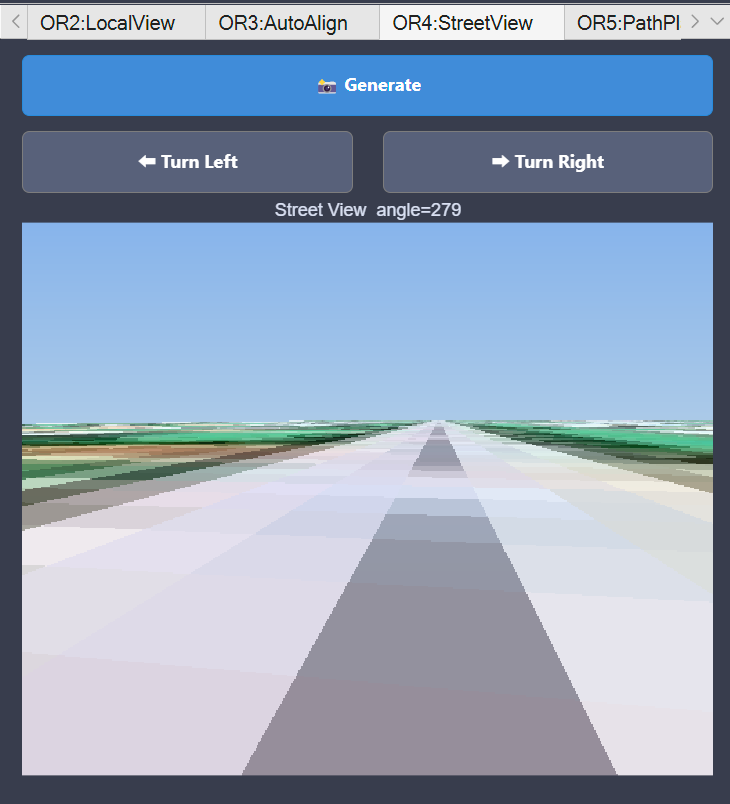
\includegraphics[width=0.92\textwidth]{uid_report_images/image_15.png}
  \caption{OR4 result: left-turn virtual street view.}
  \label{fig:or4b}
\end{figure}

\begin{figure}[H]
  \centering
  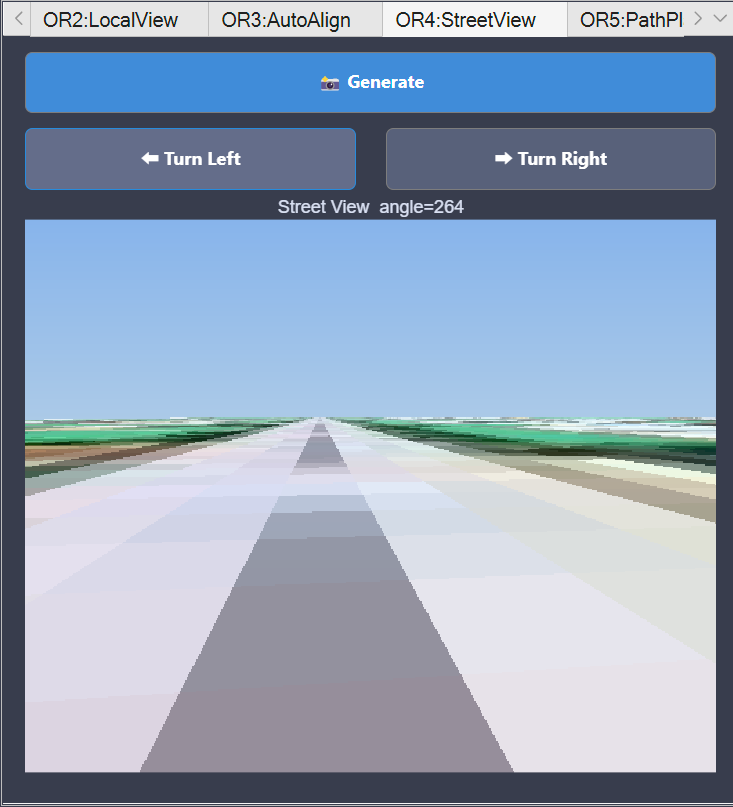
\includegraphics[width=0.92\textwidth]{uid_report_images/image_16.png}
  \caption{OR4 result: right-turn virtual street view.}
  \label{fig:or4c}
  \caption*{Note: This figure shows the OR4 virtual street-view function. The middle image is the original view, the left image is the left-turn view, and the right image is the right-turn view. This figure shows that OR4 supports street-view generation and direction adjustment.}
\end{figure}

\subsection{OR5: Path Planning}
\label{sec:or5}

\textbf{Responsible member: 李昱辰 R32314003}

Function description:

Computes and visualizes the shortest road path between two user-selected points by snapping them to the nearest road pixels and performing BFS on the road mask.

Implementation idea:

The OR5 panel lets the user click start and destination points anywhere on the map. Each point is snapped to the nearest road pixel in the road mask. Then a BFS over the 8-connected road pixel graph produces a shortest path, which is reconstructed and visualized.

Key parameters / data:

Road mask: \texttt{roadMask}

Connectivity: 8-connected neighbourhood (3×3)

Snapping search radius limit: $r_\text{max}$ (pixels)

BFS predecessor array: \texttt{prev}

Processing pipeline:

\begin{enumerate}
  \item User input

  Start click $(u_s, v_s)$, target click $(u_t, v_t)$.

  \item Snap-to-road (for each point)

  If clicked pixel is not road, search outward until a road pixel is found:

  practical approach: BFS/ring expansion around click

  Output snapped points $(u_s', v_s')$, $(u_t', v_t')$.

  \item Shortest path BFS on road graph

  Nodes: all pixels where \texttt{roadMask=true}.

  Edges: 8-connected neighbours.

  BFS from start to target, store predecessor: \texttt{prev[next]=cur}.

  \item Path reconstruction

  Backtrack from target to start using \texttt{prev} to obtain a pixel path sequence.

  \item Visualization

  Render the path as a coloured polyline overlay on the main map.
\end{enumerate}

How to use:

\begin{enumerate}
  \item Open OR5 tab $\rightarrow$ Click Start Path
  \item Click start point $\rightarrow$ Click destination point
  \item System computes and shows shortest path
  \item Click Clear to reset
\end{enumerate}

Representative results of OR5 are shown in Figures~\ref{fig:or5a} and \ref{fig:or5b}.

\begin{figure}[H]
  \centering
  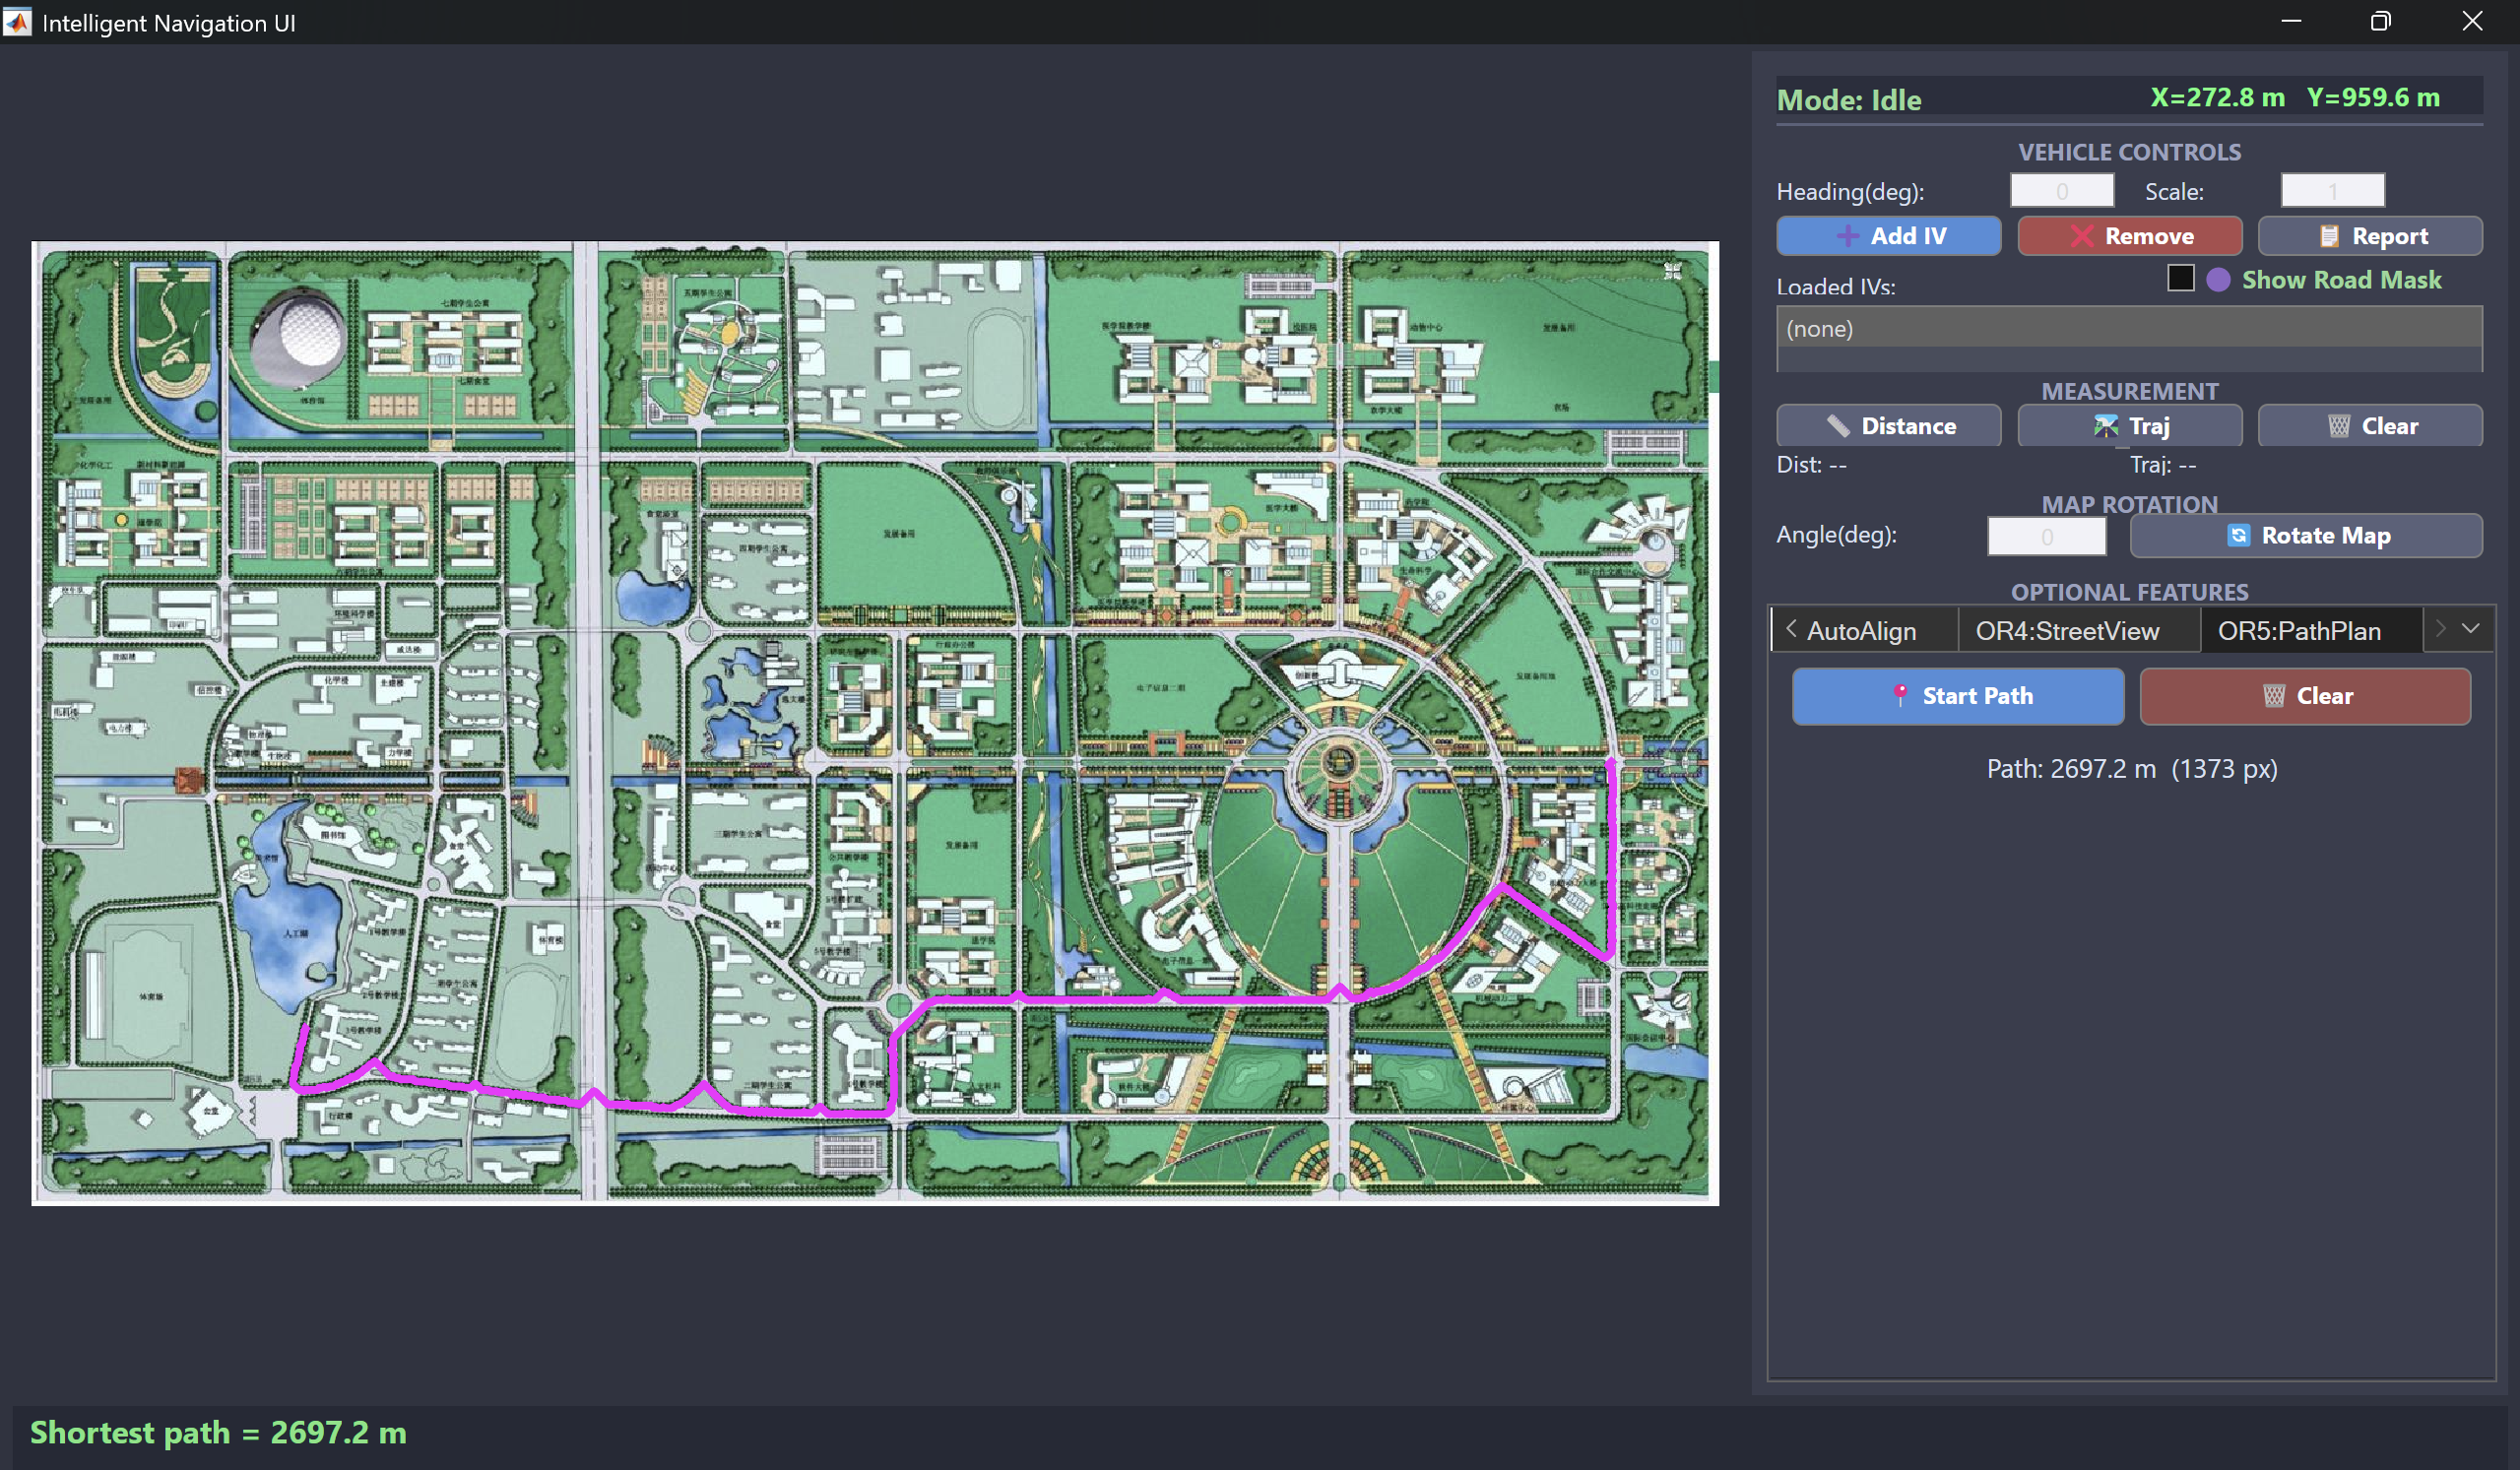
\includegraphics[width=0.92\textwidth]{uid_report_images/image_17.png}
  \caption{OR5 result: shortest-path planning example 1.}
  \label{fig:or5a}
\end{figure}

\begin{figure}[H]
  \centering
  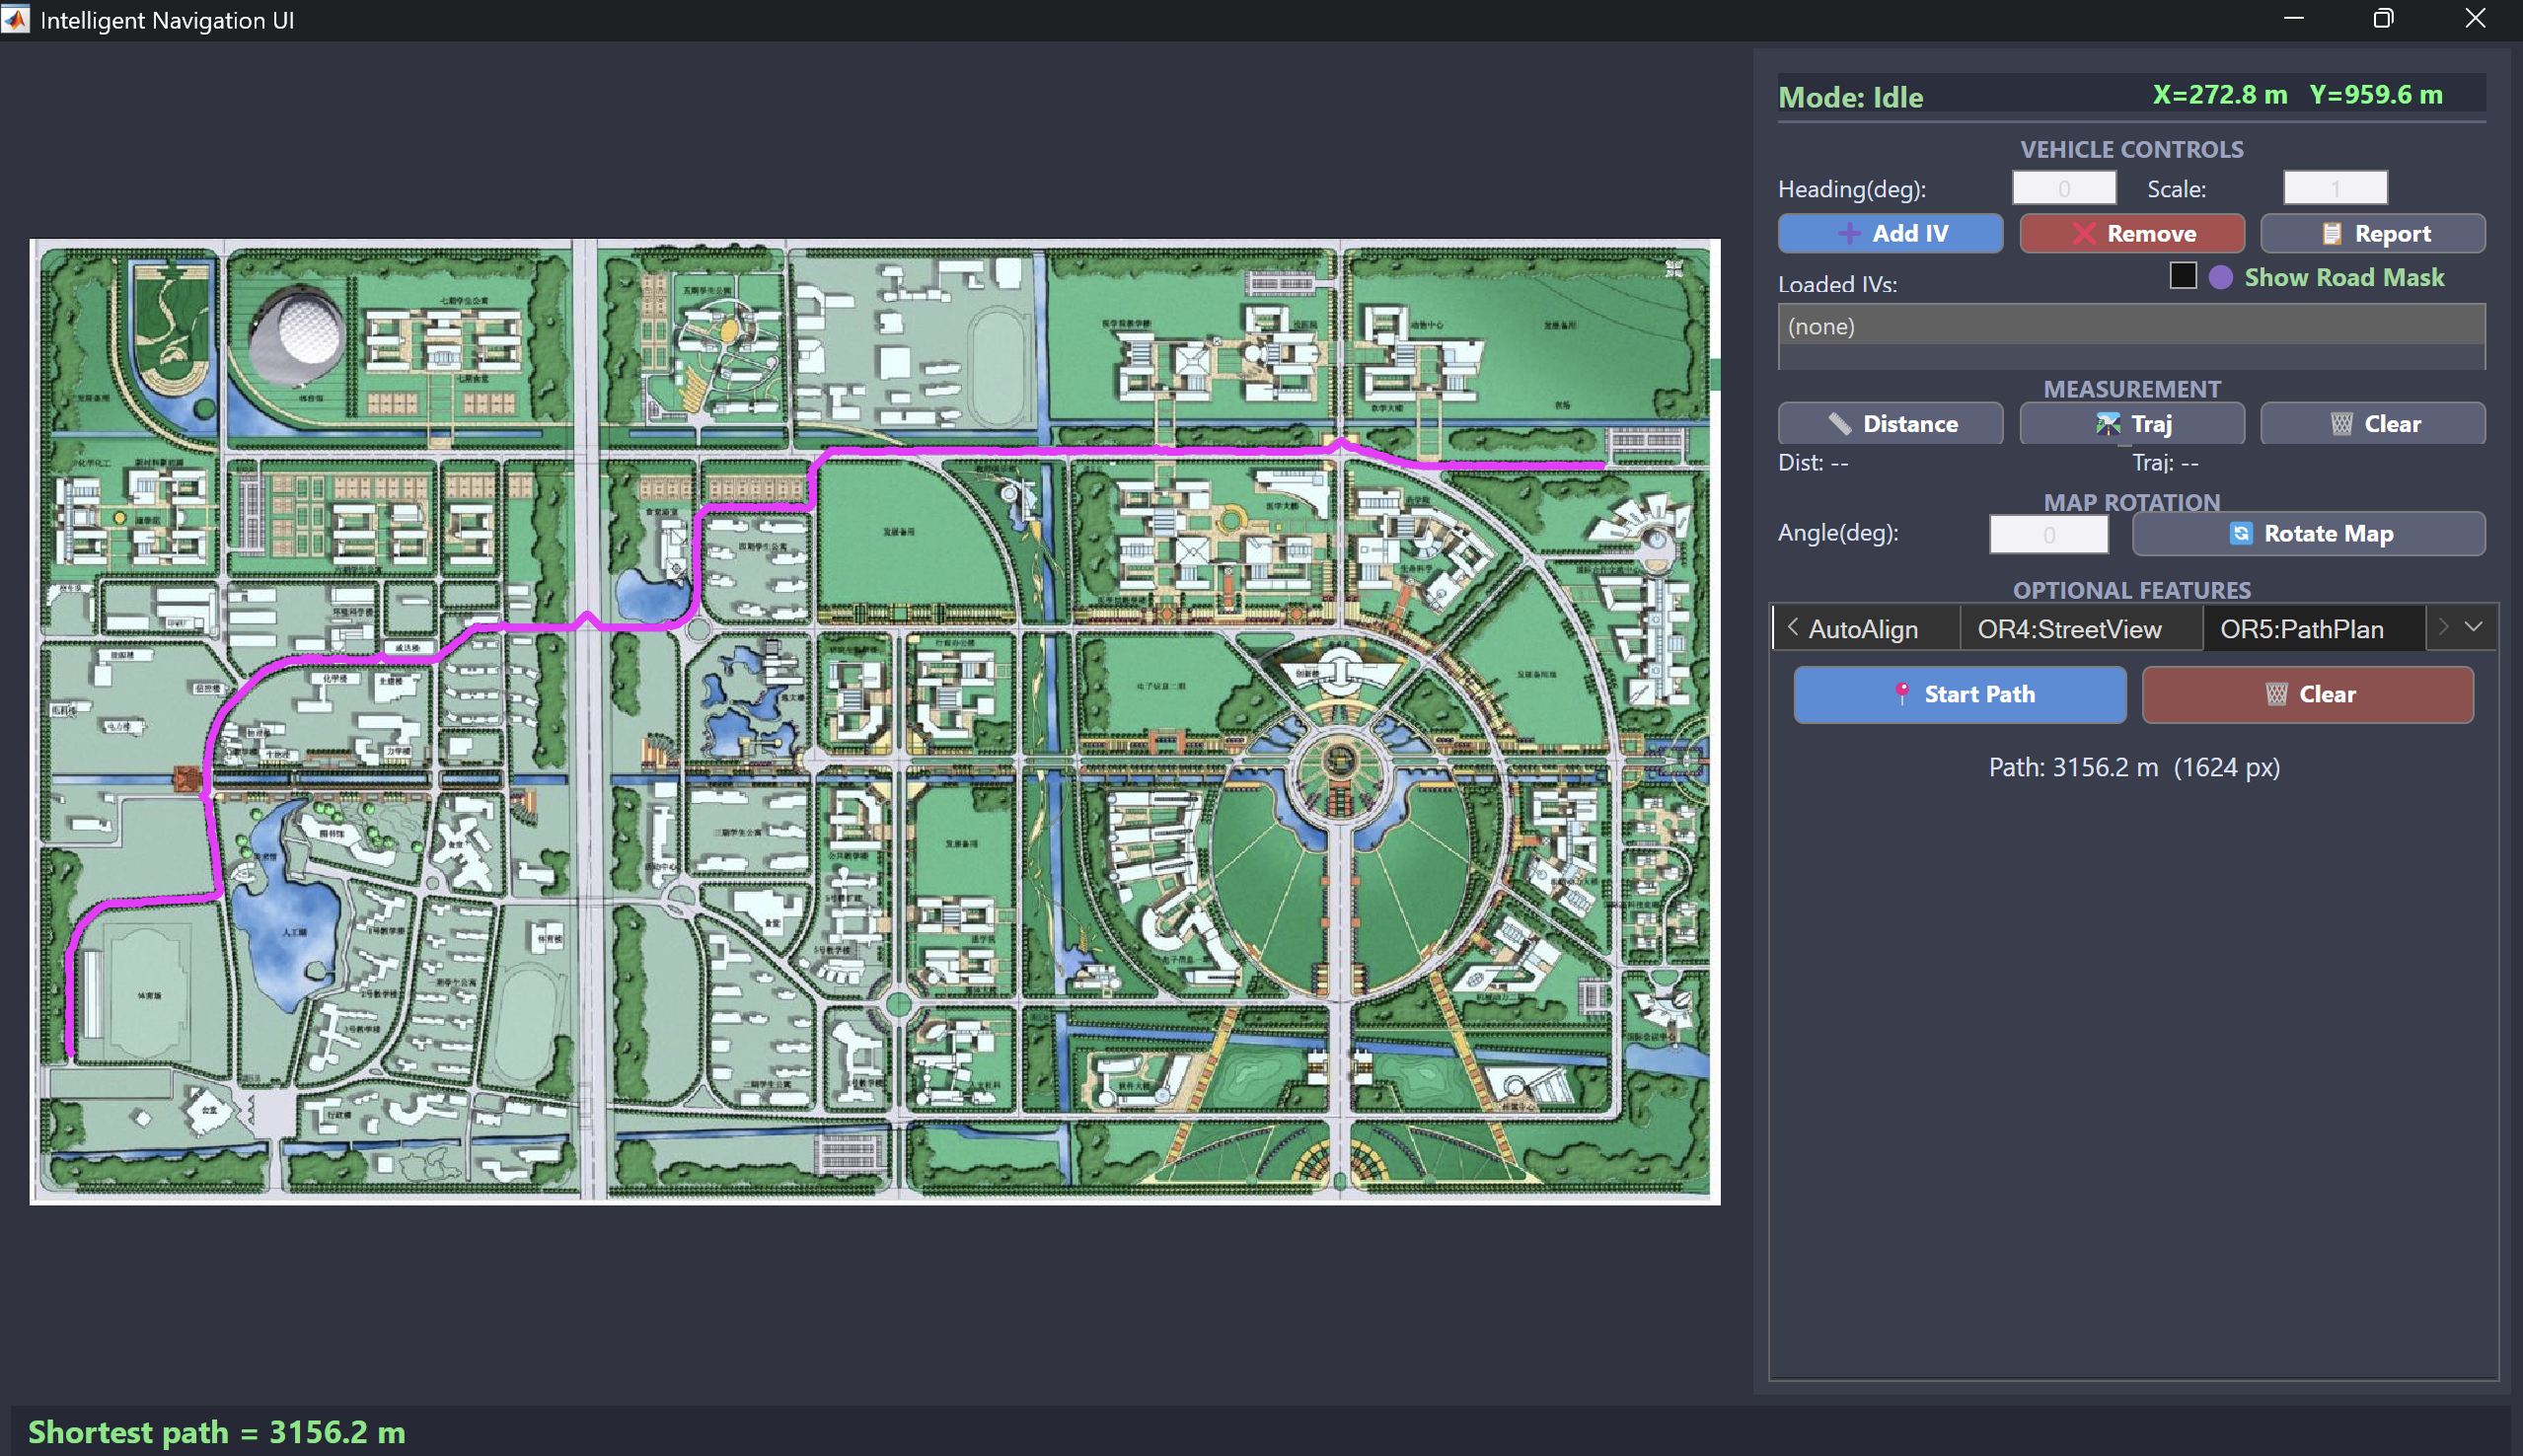
\includegraphics[width=0.92\textwidth]{uid_report_images/image_18.png}
  \caption{OR5 result: shortest-path planning example 2.}
  \label{fig:or5b}
  \caption*{Note: This figure shows two examples of the OR5 shortest-path planning result. In both cases, the system computes the road-based shortest path between the selected points and displays it as a highlighted path on the map. The total path length is also shown in the panel. This figure demonstrates that OR5 supports shortest-path planning and path visualization.}
\end{figure}

\section{User Guide}

\subsection{How to Start the System}

Open MATLAB.

Open the project folder.

Run the main script main.m.

Wait for the UI window to appear.

\subsection{How to Add an IV}

Input the heading angle.

Input the scale factor.

Click Add IV.

Click a valid road point on the map.

\subsection{How to Remove an IV}

Select an IV from the list.

Click Remove.

\subsection{How to Measure Distance}

Click Distance.

Click two points on the map.

Read the result from the map and the right panel.

\subsection{How to Measure Trajectory}

Click Traj.

Click multiple points continuously on the map.

Read the accumulated trajectory length from the right panel.

\subsection{How to Rotate the Map}

Input the rotation angle.

Click Rotate Map.

\subsection{How to Use Optional Functions}

OR1: Go to the OR1 tab, click Extract, click road points, click End, click Show Skel or Road Area, and click Clear if needed.

OR2: Go to the OR2 tab, load IVs, select an IV, input the range (m), click Update, and click Show Direction or Hide Direction if needed.

OR3: Go to the OR3 tab, click Auto-Add IV, click a road point, select an IV, click Head-Up View, and click Normal View to restore.

OR4: Go to the OR4 tab, click Generate, and click a road point on the map to display the street view.

OR5: Go to the OR5 tab, click Start Path, click the start point, click the destination point, view the shortest path overlay, and click Clear if needed.

\section{Group Work Distribution}

Member Name | Student ID | Responsibility

李昱辰 | R32314003

Engineered the initial UI framework, defining the core graphical canvas, event listening structures, and base data structures for IV management.

Implemented interactive start/end node selection on the road grid; developed the network pathfinding algorithm to compute optimal trajectories; integrated cumulative distance calculations and dynamic route highlight rendering.

OR5: Path Planning

王瑞尧 | R32314007

Optimized UI core architecture and user interaction logic after the initial draft.

Developed a local road direction estimator using neighborhood mask sampling; engineered "Head-Up View" for map rotation around the active IV and "Normal View" for restoring north-up orientation. Designed an explicit vehicle heading indicator to ensure the auto-alignment is intuitive for evaluation.

OR3: IV Automatic Orientation Alignment

刘江翰 | R32314009

Optimized the overall UI layout and resolved text-overlapping issues, fixed the distance label occluding the two endpoints and fixed an issue where the distance label and trajectory overlay did not rotate together with the map.

OR2: Scale and Local Visualization

纪玮祺 | R32314005

Evaluated multi-version UI designs based on project requirements to define clear optimization paths.

deeply optimized the road detection algorithm, successfully achieving almost 100\% recall rate.

OR4: Virtual Street View Generation

刘熙鹏 | R32314091

Managed final UI integration, error handling for interactive coordinates, and multi-panel system stability.

Implemented interactive polyline skeleton extraction via centerline clicking; supported independent skeleton rendering in real-world coordinates and dynamic isolation/highlighting of neighboring drivable road patches.

OR1: Road Skeleton Extraction

\section{Requirement Checklist}

\begin{figure}[H]
  \centering
  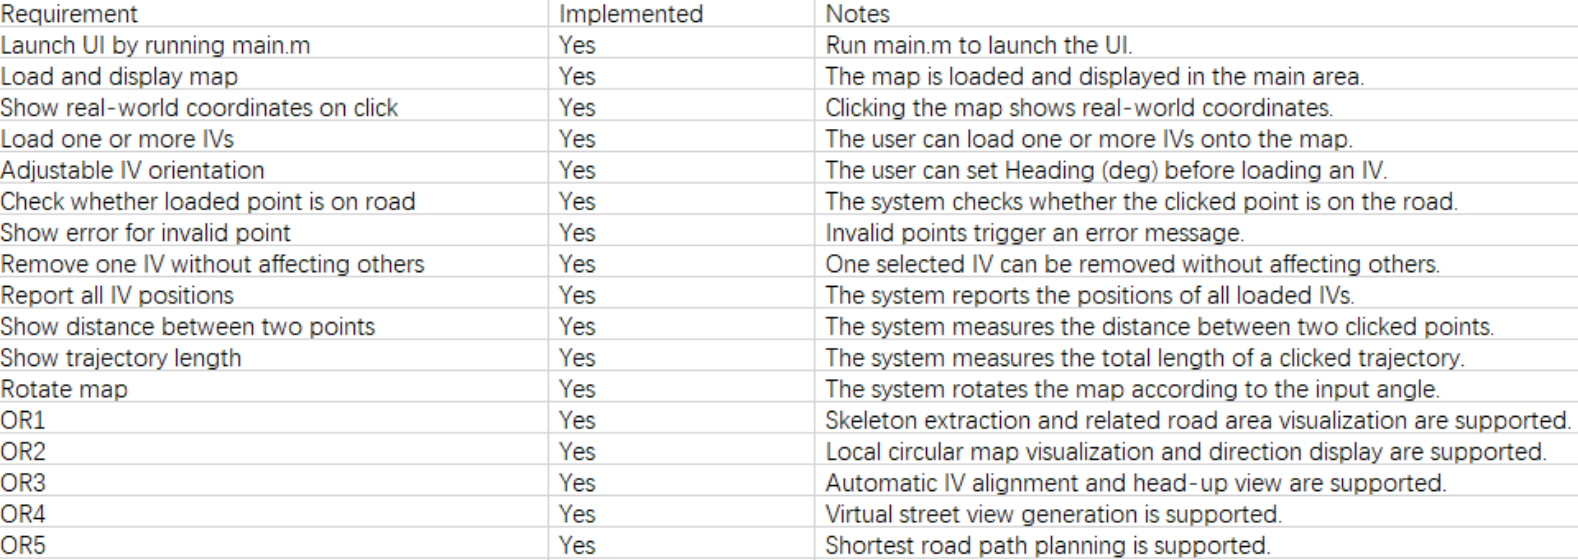
\includegraphics[width=0.92\textwidth]{uid_report_images/image_01.png}
  \label{fig:checklist}
\end{figure}

\section{Conclusion}

This project implements an Intelligent Navigation UI in MATLAB according to the course requirements. The system supports map visualization, IV loading, coordinate display, distance and trajectory measurement, map rotation, and all five optional functions. The GUI-based design makes the system easy to use and suitable for demonstrating the required functions of the course project.

Details of the optional functions and group contributions are presented in the corresponding sections above.

\section{Appendix}

\subsection{Project Files}

main.m

src/

MapForUI.jpg

README.md

UID\_CourseProject.pdf

\end{document}
